\documentclass[
]{jss}

%% recommended packages
\usepackage{orcidlink,thumbpdf,lmodern}

\usepackage[utf8]{inputenc}

\author{
Brian J. Smith\\Department of Biostatstics \And Stephen L.
Hillis\\Departments of Radiology and Biostatsitics
}
\title{\pkg{MRMCaov}: Multi-Reader Multi-Case ANOVA Software for
\proglang{R}}

\Plainauthor{Brian J. Smith, Stephen L. Hillis}
\Plaintitle{MRMCaov: Multi-Reader Multi-Case ANOVA Software for R}
\Shorttitle{\pkg{MRMCaov}}


\Abstract{
The abstract of the article.
}

\Keywords{keywords, not capitalized, \proglang{Java}}
\Plainkeywords{keywords, not capitalized, Java}

%% publication information
%% \Volume{50}
%% \Issue{9}
%% \Month{June}
%% \Year{2012}
%% \Submitdate{}
%% \Acceptdate{2012-06-04}

\Address{
    Brian J. Smith\\
    Department of Biostatstics\\
    University of Iowa,\\
Iowa City, Iowa, USA\\
  E-mail: \email{brian-j-smith@uiowa.edu}\\
  
      Stephen L. Hillis\\
    Departments of Radiology and Biostatsitics\\
    University of Iowa,\\
Iowa City, Iowa, USA\\
  E-mail: \email{steve-hillis@uiowa.edu}\\
  
  }


% tightlist command for lists without linebreak
\providecommand{\tightlist}{%
  \setlength{\itemsep}{0pt}\setlength{\parskip}{0pt}}



\usepackage{amsmath}
\usepackage{booktabs}
\usepackage[most]{tcolorbox}

\newenvironment{Description}{\textbf{Description}\vspace{0.5em}\newline}{\vspace{0.5em}\newline}

\newtcolorbox[auto counter,number within=section]{example}[2][]{
  enhanced,
  breakable,
  title={MATLAB Example \thetcbcounter: #2},
  #1
}



\begin{document}



\hypertarget{introduction}{%
\section{Introduction}\label{introduction}}

A common study design for comparing the diagnostic performance of
imaging modalities, or diagnostic tests, is to obtain modality-specific
ratings from multiple readers of multiple cases (MRMC) whose true
statuses are known. In such a design, receiver operating characteristic
(ROC) metrics, such as area under the ROC curve (ROC AUC), can be used
to quantify correspondence between reader ratings and case status.
Metrics can then be compared statistically to determine if modalities
differ. However, special statistical methods are needed when readers or
cases represent a random sample from a larger population of interest and
there is overlap between modalities, readers, and/or cases. An ANOVA
model designed for these characteristics of MRMC studies was initially
proposed by Dorfman et al. \citep{Dorfman:1992:ROC} and Obuchowski and
Rockette \citep{Obuchowski:1995:HTD} and later unified and improved by
Hillis and colleagues
\citep{Hillis:2005:CDB, Hillis:2007:CDD, Hillis:2008:RDD, Hillis:2018:RRM}.
This paper describes the implementation of their models in the
\pkg{MRMCaov} \proglang{R} package \citep{MRMCaov-package}.

Several other \proglang{R} packages allow for the estimation and
comparison of certain ROC metrics and MRMC study designs. \pkg{pROC}
provides general tools for the estimation, visualization, and comparison
of ROC AUC and sensitivity/specificity at a given
specificity/sensitivity \citep{Robin:2011:pROC}. The package can be used
to compare these metrics across two diagnostic tests in MRMC study
designs where one reader rates the same (paired) or different (unpaired)
sets of cases. \pkg{iMRMC} is specifically designed to compare ROC AUC,
sensitivity, and specificity in MRMC studies of two or more diagnostic
tests \citep{Gallas:2022:iMRMC}. Arbitrary study designs are supported
in which one or more readers provide ratings that are paired, unpaired,
or partially paired (some combination thereof). The package is based on
a U-statistics approach to estimating the metrics and their covariances.
\pkg{RJafroc} enables analysis of ROC free-response receiver operating
characteristic (FROC) curves across one or more diagnostic tests in MRMC
studies, and \pkg{BayesianFROC} is a Bayesian implementation of FROC
methods.

\hypertarget{obuchowski-and-rockette-model}{%
\section{Obuchowski and Rockette
Model}\label{obuchowski-and-rockette-model}}

\pkg{MRMCaov} implements multi-reader multi-case analysis based on the
Obuchowski and Rockette \citeyearpar{Obuchowski:1995:HTD} analysis of
variance (ANOVA) model \[
\hat{\theta}_{ij} = \mu + \tau_i + R_j + (\tau R)_{ij} + \epsilon_{ij},
\] where \(i = 1,\ldots,t\) and \(j = 1,\ldots,r\) index diagnostic
tests and readers; \(\hat{\theta}_{ij}\) is a reader performance metric,
such as ROC AUC, estimated over multiple cases; \(\mu\) an overall study
mean; \(\tau_i\) a fixed test effect; \(R_j\) a random reader effect;
\((\tau R)_{ij}\) a random test \(\times\) reader interaction effect;
and \(\epsilon_{ij}\) a random error term. The random terms \(R_j\),
\((\tau R)_{ij}\), and \(\epsilon_{ij}\) are assumed to be mutually
independent and normally distributed with 0 means and variances
\(\sigma^2_R\), \(\sigma^2_{TR}\), and \(\sigma^2_\epsilon\).

The error covariances between tests and between readers are further
assumed to be equal, resulting in the three covariances \[
\text{Cov}(\epsilon_{ij}, \epsilon_{i'j'}) = \left\{
  \begin{array}{lll}
    \text{Cov}_1 & i \ne i', j = j' & \text{(different test, same reader)} \\
    \text{Cov}_2 & i = i', j \ne j' & \text{(same test, same reader)} \\
    \text{Cov}_3 & i \ne i', j \ne j' & \text{(different test, different reader)}.
  \end{array}
\right.
\] Obuchowski and Rockette \citeyearpar{Obuchowski:1995:HTD} suggest a
covariance ordering of
\(\text{Cov}_1 \ge \text{Cov}_2 \ge \text{Cov}_3 \ge 0\) based on
clinical considerations. Hillis \citeyearpar{Hillis:2014:MMA} later
showed that these can be replaced with the less restrictive orderings
\(\text{Cov}_1 \ge \text{Cov}_3\), \(\text{Cov}_2 \ge \text{Cov}_3\),
and \(\text{Cov}_3 \ge 0\). Alternatively, the covariance can be
specified as the population correlations
\(\rho_i = \text{Cov}_i / \sigma^2_\epsilon\).

In the Obuchowski-Rockette ANOVA model, \(\sigma^2_\epsilon\) can be
interpreted as the performance metric variance for a single fixed reader
and test; and \(\text{Cov}_1\), \(\text{Cov}_2\), and \(\text{Cov}_3\)
as the performance metric covariances for the same reader of two
different tests, two different readers of the same test, and two
different readers of two different tests. These error variance and
covariance parameters are estimated in the package by averaging the
reader and test-specific estimates computed using jackknifing
\citep{Efron:1982:JBR} or, for empirical ROC AUC, an unbiased estimator
\citep{Gallas:2007:MMV} or the method of DeLong \citep{DeLong:1988:CAU}.

Hillis \citeyearpar{Hillis:2014:MMA} developed a framework in which the
the Obuchowski-Rockette model can be viewed generally as a marginal-mean
ANOVA model. His framework provides easy derivations of test statistics
and parameter estimates, as well as their distributions and confidence
intervals; allows for easy generalization to nested study designs; and
is the basis for MRMC analysis in the package. In particular, package
analyses return test statistics and p-values for a global test of
equality of reader performances across all diagnostic tests and for
tests of their pairwise differences. Also returned are estimates of test
performances and performance differences along with their confidence
intervals. Moreover, the framework enables support for paired, unpaired,
or partially paired study designs and for the designation of readers or
cases as fixed instead of random.

\hypertarget{vandyke-example}{%
\section{VanDyke Example}\label{vandyke-example}}

Use of the \pkg{MRMCaov} package is illustrated with data from a study
comparing the relative performance of cinematic presentation of MRI
(CINE MRI) to single spin-echo magnetic resonance imaging (SE MRI) for
the detection of thoracic aortic dissection \citep{VanDyke:1993:CMD}. In
the study, 45 patients with aortic dissection and 69 without dissection
were imaged with both modalities. Based on the images, five radiologists
rated patients disease statuses as 1 = definitely no aortic dissection,
2 = probably no aortic dissection, 3 = unsure about aortic dissection, 4
= probably aortic dissection, or 5 = definitely aortic dissection.
Interest lies in estimating ROC curves for each combination of reader
and modality and in comparing modalities with respect to summary
statistics from the curves. The study data are included in the package
as a data frame named \texttt{VanDyke}.

\begin{CodeChunk}
\begin{CodeInput}
R> ## Load MRMCaov library and VanDyke dataset
R> library(MRMCaov)
R> data(VanDyke, package = "MRMCaov")
\end{CodeInput}
\end{CodeChunk}

\begin{CodeChunk}
\begin{CodeOutput}
   reader treatment case truth rating case2 case3
1       1         1    1     0      1   1.1   1.1
2       1         2    1     0      3   1.1   2.1
3       2         1    1     0      2   2.1   1.1
4       2         2    1     0      3   2.1   2.1
5       3         1    1     0      2   3.1   1.1
6       3         2    1     0      2   3.1   2.1
7       4         1    1     0      1   4.1   1.1
8       4         2    1     0      2   4.1   2.1
9       5         1    1     0      3   5.1   1.1
10      5         2    1     0      2   5.1   2.1
11      1         1    2     0      2   1.2   1.2
12      1         2    2     0      3   1.2   2.2
13      2         1    2     0      3   2.2   1.2
14      2         2    2     0      2   2.2   2.2
15      3         1    2     0      2   3.2   1.2
16      3         2    2     0      4   3.2   2.2
17      4         1    2     0      1   4.2   1.2
18      4         2    2     0      2   4.2   2.2
19      5         1    2     0      5   5.2   1.2
20      5         2    2     0      2   5.2   2.2
... with 1120 more rows
\end{CodeOutput}
\end{CodeChunk}

The study employed a factorial design in which each of the five
radiologists read and rated both the CINE and SE MRI images from all 114
cases. The original study variables in the \texttt{VanDyke} data frame
are summarized in Table\textasciitilde{}\ref{tbl:VanDyke} along with two
additional \texttt{case2} and \texttt{case3} variables that represent
hypothetical study designs in which cases are nested within readers
(\texttt{reader}) and within imaging modalities (\texttt{treatment}),
respectively.

\begin{table}[h]
\caption{VanDyke study variables}
\label{tbl:VanDyke}
\begin{tabular}{ll}
\toprule
Variable    & Description \\
\midrule
\code{reader}    & unique identifiers for the five radiologists                                \\
\code{treatment} & identifiers for the imaging modality (1 = CINE MRI, 2 = SE MRI)             \\
\code{case}      & identifiers for the 114 cases                                               \\
\code{truth}     & indicator for thoracic aortic dissection (1 = performed, 0 = not performed) \\
\code{rating}    & five-point ratings given to case images by the readers                      \\
\code{case2}     & example identifiers representing nesting of cases within readers            \\
\code{case3}     & example identifiers representing nesting of cases within treatments         \\
\bottomrule
\end{tabular}
\end{table}

Data from other studies may be analyzed with the package and should
follow the format of \texttt{VanDyke} with columns for reader,
treatment, and case identifiers as well as true event statuses and
reader ratings. The variable names, however, may be different.

\hypertarget{multi-reader-multi-case-analysis}{%
\section{Multi-Reader Multi-Case
Analysis}\label{multi-reader-multi-case-analysis}}

A multi-reader multi-case (MRMC) analysis, as the name suggests,
involves multiple readers of multiple cases to compare reader
performance metrics across two or more diagnostic tests. An MRMC
analysis can be performed with a call to the \texttt{mrmc()} function to
specify a reader performance metric, study variables and observations,
and covariance estimation method.

\begin{tcolorbox}[title=MRMC Function]
\textbf{Syntax}
\begin{verbatim}
mrmc(response, test, reader, case, data, cov = jackknife)
\end{verbatim}
\begin{Description}
Returns an \code{mrmc} class object of data that can be used to estimate and compare reader performance metrics in a multi-reader multi-case statistical analysis.
\end{Description}
\textbf{Arguments}
\begin{description}
\item[\code{response}:] object defining true case statuses, corresponding reader ratings, and a reader performance metric to compute on them.
\item[\code{test}, \code{reader}, \code{case}:] variables containing the test, reader, and case identifiers for the \code{response} observations.
\item[\code{data}:] data frame containing the response and identifier variables.
\item[\code{cov}:] function \code{jackknife}, \code{unbiased}, or \code{DeLong} to estimate reader performance metric covariances.
\end{description}
\end{tcolorbox}

The response variable in the \texttt{mrmc()} specification is defined
with one of the performance metrics described in the following sections.
Results from \texttt{mrmc()} can be displayed with \texttt{print()} and
passed to \texttt{summary()} for statistical comparisons of the
diagnostic tests. The summary call produces ANOVA results from a global
test of equality of ROC AUC means across all tests and statistical tests
of pairwise differences, along with confidence intervals for the
differences and intervals for individual tests.

\begin{tcolorbox}[title=MRMC Summary Function]
\textbf{Syntax}
\begin{verbatim}
summary(object, conf.level = 0.95)
\end{verbatim}
\begin{Description}
Returns a \code{summary.mrmc} class object of statistical results from a multi-reader multi-case analysis.
\end{Description}
\textbf{Arguments}
\begin{description}
\item[\code{object}:] results from \code{mrmc()}.
\item[\code{conf.level}:] confidence level for confidence intervals.
\end{description}
\end{tcolorbox}

\hypertarget{performance-metrics}{%
\subsection{Performance Metrics}\label{performance-metrics}}

\hypertarget{area-under-the-roc-curve}{%
\subsubsection{Area Under the ROC
Curve}\label{area-under-the-roc-curve}}

Area under the ROC curve is a measure of concordance between numeric
reader ratings and true binary case statuses. It provides an estimate of
the probability that a randomly selected positive case will have a
higher rating than a negative case. ROC AUC values range from 0 to 1,
with 0.5 representing no concordance and 1 perfect concordance. AUC can
be computed with the functions described below for binormal, binormal
likelihood-ratio, and empirical ROC curves. Empirical curves are also
referred to as trapezoidal. The functions also support calculation of
partial AUC over a range of sensitivities or specificities.

\begin{tcolorbox}[title=ROC AUC Functions]
\textbf{Syntax}
\begin{footnotesize}
\begin{verbatim}
binormal_auc(truth, rating, partial = FALSE, min = 0, max = 1, normalize = FALSE) 
binormalLR_auc(truth, rating, partial = FALSE, min = 0, max = 1, normalize = FALSE)
empirical_auc(truth, rating, partial = FALSE, min = 0, max = 1, normalize = FALSE) 
trapezoidal_auc(truth, rating, partial = FALSE, min = 0, max = 1, normalize = FALSE)
\end{verbatim}
\end{footnotesize}
\begin{Description}
Returns computed area under the receiver operating character curve estimated with a binormal model (\code{binormal\_auc}), binormal likelihood-ratio model (\code{binormalLR\_auc}), or empirically (\code{empirical\_auc} or \code{trapezoidal\_auc}).
\end{Description}
\textbf{Arguments}
\begin{description}
\item[\code{truth}:] vector of true binary case statuses, with positive status taken to be the highest level.
\item[\code{rating}:] numeric vector of case ratings.
\item[\code{partial}:] character string \code{"sensitivity"} or \code{"specificity"} for calculation of partial AUC, or \code{FALSE} for full AUC.  Partial matching of the character strings is allowed.  A value of \code{"specificity"} results in area under the ROC curve between the given \code{min} and \code{max} specificity values, whereas \code{"sensitivity"} results in area to the right of the curve between the given sensitivity values.
\item[\code{min}, \code{max}:] minimum and maximum sensitivity or specificity values over which to calculate partial AUC.
\item[\code{normalize}:] logical indicating whether partial AUC is divided by the interval width (\code{max - min}) over which it is calculated.
\end{description}
\end{tcolorbox}

In the example below, \texttt{mrmc()} is called to compare CINE MRI and
SE MRI treatments in an MRMC analysis of areas under binormal ROC curves
computed for the readers of cases in the VanDyke study.

\begin{CodeChunk}
\begin{CodeInput}
R> ## Compare ROC AUC treatment means for the VanDyke example
R> est <- mrmc(
+   binormal_auc(truth, rating), treatment, reader, case, data = VanDyke
+ )
\end{CodeInput}
\end{CodeChunk}

The \texttt{print()} function can be applied to \texttt{mrmc()} output
to display information about the reader performance metrics, including
the

\begin{itemize}
\tightlist
\item
  value of variable \texttt{truth} (1) defining positive case status,
\item
  estimated performance metric values (\texttt{data\$binormal\_auc}) for
  each test (\texttt{\$treatment}) and reader (\texttt{\$reader}),
\item
  number of cases read at each level of the factors (\texttt{N}), and
\item
  error variance \(\sigma^2_\epsilon\) and covariances \(\text{Cov}_1\),
  \(\text{Cov}_2\), and \(\text{Cov}_3\).
\end{itemize}

\textbf{MRMC Performance Metrics}

\begin{CodeChunk}
\begin{CodeInput}
R> print(est)
\end{CodeInput}
\begin{CodeOutput}
Call:
mrmc(response = binormal_auc(truth, rating), test = treatment, 
    reader = reader, case = case, data = VanDyke)

Positive truth status: 1 

Response metric data:

# A tibble: 10 x 2
       N data$binormal_auc $treatment $reader
   <dbl>             <dbl> <fct>      <fct>  
 1   114             0.933 1          1      
 2   114             0.890 1          2      
 3   114             0.929 1          3      
 4   114             0.970 1          4      
 5   114             0.833 1          5      
 6   114             0.951 2          1      
 7   114             0.935 2          2      
 8   114             0.928 2          3      
 9   114             1     2          4      
10   114             0.945 2          5      

ANOVA Table:

                 Df    Sum Sq   Mean Sq
treatment         1 0.0041142 0.0041142
reader            4 0.0104324 0.0026081
treatment:reader  4 0.0037916 0.0009479


Obuchowski-Rockette error variance and covariance estimates:

          Estimate Correlation
Error 0.0010790449          NA
Cov1  0.0003125019   0.2896097
Cov2  0.0003116050   0.2887785
Cov3  0.0001937700   0.1795755
\end{CodeOutput}
\end{CodeChunk}

MRMC statistical tests are performed with a call to \texttt{summary()}.
Results include a test of the global null hypothesis that performances
are equal across all diagnostic tests, tests of their pairwise mean
differences, and estimated mean performances for each one.

\textbf{MRMC Test Results}

\begin{CodeChunk}
\begin{CodeInput}
R> summary(est)
\end{CodeInput}
\begin{CodeOutput}
Multi-Reader Multi-Case Analysis of Variance
Data: VanDyke
Factor types: Random Readers and Random Cases
Covariance method: jackknife

Experimental design: factorial 

Obuchowski-Rockette variance component and covariance estimates:

                     Estimate Correlation
reader           0.0007113780          NA
treatment:reader 0.0002991817          NA
Error            0.0010790449          NA
Cov1             0.0003125019   0.2896097
Cov2             0.0003116050   0.2887785
Cov3             0.0001937700   0.1795755


ANOVA global test of equal treatment binormal_auc:
        MS(T)      MS(T:R)        Cov2       Cov3 Denominator       F df1
1 0.004114199 0.0009478898 0.000311605 0.00019377 0.001537064 2.67666   1
       df2   p-value
1 10.51789 0.1313682


95% CIs and tests for treatment binormal_auc pairwise differences:
  Comparison    Estimate     StdErr       df    CI.Lower    CI.Upper        t
1      1 - 2 -0.04056698 0.02479568 10.51789 -0.09544867  0.01431471 -1.63605
    p-value
1 0.1313682


95% treatment binormal_auc CIs (each analysis based only on data for the
specified treatment):
   Estimate        MS(R)         Cov2     StdErr       df  CI.Lower  CI.Upper
1 0.9109867 0.0027417481 0.0004612327 0.03177392 13.55902 0.8426298 0.9793435
2 0.9515536 0.0008142512 0.0001619773 0.01802297 15.91435 0.9133299 0.9897774
\end{CodeOutput}
\end{CodeChunk}

ROC curves estimated by \texttt{mrmc()} can be displayed with
\texttt{plot()} and their parameters extracted with
\texttt{parameters()}.

\textbf{MRMC ROC Curves}

\begin{CodeChunk}
\begin{CodeInput}
R> plot(est)
\end{CodeInput}


\begin{center}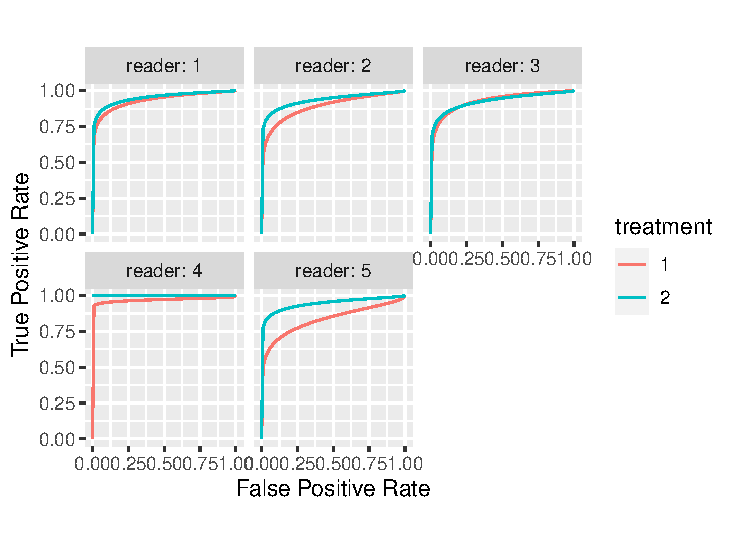
\includegraphics{MRMCaov_files/figure-latex/unnamed-chunk-13-1} \end{center}

\end{CodeChunk}

\textbf{MRMC ROC Curve Parameters}

\begin{CodeChunk}
\begin{CodeInput}
R> print(parameters(est))
\end{CodeInput}
\begin{CodeOutput}
# A tibble: 10 x 3
   Group$reader $treatment        a     b
   <fct>        <fct>         <dbl> <dbl>
 1 1            1          1.70e  0 0.537
 2 2            1          1.40e  0 0.561
 3 3            1          1.74e  0 0.635
 4 4            1          1.93e  0 0.202
 5 5            1          1.06e  0 0.464
 6 1            2          1.85e  0 0.503
 7 2            2          1.66e  0 0.447
 8 3            2          1.62e  0 0.488
 9 4            2          1.80e308 1    
10 5            2          1.73e  0 0.422
\end{CodeOutput}
\end{CodeChunk}

\hypertarget{roc-curve-expected-utility}{%
\subsubsection{ROC Curve Expected
Utility}\label{roc-curve-expected-utility}}

As an alternative to AUC as a summary of ROC curves, Abbey et
al.~{[}-Aabbey:2013:SPC{]} propose an expected utility metric defined as
\[
\text{EU} = \max_\text{FPR}(\text{TPR}(\text{FPR}) - \beta \times \text{FPR}),
\] where \(\text{TPR}(\text{FPR})\) are true positive rates on the ROC
curve, and FPR are false positive rates ranging from 0 to 1. From a
decision theory perspective, expected utility can be viewed as the
expected loss of classifying cases and is minimized when
\(\beta = (1 - p) / (r \times p)\), where \(p\) is the population
prevalence of positive cases and \(r\) is the cost associated with a
false negative classification relative to a false positive one
\citep{Perkins:2006:IOC}. Accordingly, expected utility could be used to
compare diagnostic tests with respect to the ``optimalities'\,' of their
classifications for a specified disease prevalence \(p\) and relative
cost of incorrect classifications \(r\).

\begin{tcolorbox}[title=ROC Curve Expected Utility Functions]
\textbf{Syntax}
\begin{verbatim}
binormal_eu(truth, rating, slope = 1) 
binormalLR_eu(truth, rating, slope = 1)
empirical_eu(truth, rating, slope = 1) 
trapezoidal_eu(truth, rating, slope = 1)
\end{verbatim}
\begin{Description}
Returns expected utility of an ROC curve.
\end{Description}
\textbf{Arguments}
\begin{description}
\item[truth:] vector of true binary case statuses, with positive status taken to be the highest level.
\item[\code{rating}:] numeric vector of case ratings.
\item[\code{slope}:] numeric slope ($\beta$) at which to compute expected utility.
\end{description}
\end{tcolorbox}

\hypertarget{roc-curve-sensitivity-and-specificity}{%
\subsubsection{ROC Curve Sensitivity and
Specificity}\label{roc-curve-sensitivity-and-specificity}}

Functions are provided to extract sensitivity from an ROC curve for a
given specificity and vice versa.

\begin{tcolorbox}[title=ROC Curve Sensitivity and Specificity Functions]
\textbf{Syntax}
\begin{verbatim}
binormal_sens(truth, rating, spec)
binormal_spec(truth, rating, sens)
binormalLR_sens(truth, rating, spec)
binormalLR_spec(truth, rating, sens)
empirical_sens(truth, rating, spec)
empirical_spec(truth, rating, sens)
trapezoidal_sens(truth, rating, spec)
trapezoidal_spec(truth, rating, sens)
\end{verbatim}
\begin{Description}
Returns the sensitivity/specificity from an ROC curve at a specified specificity/sensitivity.
\end{Description}
\textbf{Arguments}
\begin{description}
\item[\code{truth}:] vector of true binary case statuses, with positive status taken to be the highest level.
\item[\code{rating}:] numeric vector of case ratings.
\item[\code{spec}, \code{sens}:] specificity/sensitivity on the ROC curve at which to return sensitivity/specificity.
\end{description}
\end{tcolorbox}

\hypertarget{binary-metrics}{%
\subsubsection{Binary Metrics}\label{binary-metrics}}

Metrics for binary reader ratings are also available.

\begin{tcolorbox}[title=Sensitivity and Specificity Functions]
\textbf{Syntax}
\begin{verbatim}
binary_sens(truth, rating)
binary_spec(truth, rating)
\end{verbatim}
\begin{Description}
Returns the sensitivity or specificity.
\end{Description}
\textbf{Arguments}
\begin{description}
\item[\code{truth}:] vector of true binary case statuses, with positive status taken to be the highest level.
\item[\code{rating}:] factor or numeric vector of 0-1 binary ratings.
\end{description}
\end{tcolorbox}

\begin{CodeChunk}
\begin{CodeInput}
R> ## Compare sensitivity for binary classification
R> VanDyke$binary_rating <- VanDyke$rating >= 3
R> est <- mrmc(
+   binary_sens(truth, binary_rating), treatment, reader, case, data = VanDyke
+ )
\end{CodeInput}
\end{CodeChunk}

\textbf{MRMC Performance Metrics}

\begin{CodeChunk}
\begin{CodeInput}
R> print(est)
\end{CodeInput}
\begin{CodeOutput}
Call:
mrmc(response = binary_sens(truth, binary_rating), test = treatment, 
    reader = reader, case = case, data = VanDyke)

Positive truth status: 1 

Response metric data:

# A tibble: 10 x 2
       N data$binary_sens $treatment $reader
   <dbl>            <dbl> <fct>      <fct>  
 1    45            0.889 1          1      
 2    45            0.778 1          2      
 3    45            0.822 1          3      
 4    45            0.933 1          4      
 5    45            0.689 1          5      
 6    45            0.978 2          1      
 7    45            0.822 2          2      
 8    45            0.911 2          3      
 9    45            1     2          4      
10    45            0.889 2          5      

ANOVA Table:

                 Df   Sum Sq   Mean Sq
treatment         1 0.023901 0.0239012
reader            4 0.049679 0.0124198
treatment:reader  4 0.007210 0.0018025


Obuchowski-Rockette error variance and covariance estimates:

          Estimate Correlation
Error 0.0023681257          NA
Cov1  0.0009943883   0.4199052
Cov2  0.0010145903   0.4284360
Cov3  0.0006604938   0.2789100
\end{CodeOutput}
\end{CodeChunk}

\textbf{MRMC Test Results}

\begin{CodeChunk}
\begin{CodeInput}
R> summary(est)
\end{CodeInput}
\begin{CodeOutput}
Multi-Reader Multi-Case Analysis of Variance
Data: VanDyke
Factor types: Random Readers and Random Cases
Covariance method: jackknife

Experimental design: factorial 

Obuchowski-Rockette variance component and covariance estimates:

                     Estimate Correlation
reader           0.0049747475          NA
treatment:reader 0.0007828283          NA
Error            0.0023681257          NA
Cov1             0.0009943883   0.4199052
Cov2             0.0010145903   0.4284360
Cov3             0.0006604938   0.2789100


ANOVA global test of equal treatment binary_sens:
       MS(T)     MS(T:R)       Cov2         Cov3 Denominator        F df1
1 0.02390123 0.001802469 0.00101459 0.0006604938 0.003572952 6.689493   1
       df2    p-value
1 15.71732 0.02008822


95% CIs and tests for treatment binary_sens pairwise differences:
  Comparison    Estimate     StdErr       df   CI.Lower   CI.Upper         t
1      1 - 2 -0.09777778 0.03780451 15.71732 -0.1780371 -0.0175185 -2.586405
     p-value
1 0.02008822


95% treatment binary_sens CIs (each analysis based only on data for the
specified treatment):
   Estimate       MS(R)        Cov2     StdErr        df  CI.Lower  CI.Upper
1 0.8222222 0.009135802 0.001646465 0.05893747 14.456811 0.6961876 0.9482568
2 0.9200000 0.005086420 0.000382716 0.03741657  7.575855 0.8328691 1.0000000
\end{CodeOutput}
\end{CodeChunk}

\hypertarget{covariance-estimation-methods}{%
\subsection{Covariance Estimation
Methods}\label{covariance-estimation-methods}}

Special statistical methods are needed in MRMC analyses to estimate
covariances between performance metrics from different readers and tests
when cases are treated as a random sample and are rated by more than one
reader or evaluated with more than one test. For this estimation, the
package provides the DeLong method \citep{DeLong:1988:CAU}, jackknifing
\citep{Efron:1982:JBR}, and an unbiased method \citep{Gallas:2007:MMV}.
The applicability of each depends on the study design as well as the
performance metric being analyzed, as summarized in
Table\textasciitilde{}\ref{tbl:cov}. DeLong is appropriate for a
balanced factorial design and empirical ROC AUC, jackknifing for any
design and metric, and unbiased for any design and empirical ROC AUC.

\begin{table}
\caption{MRMC covariance estimation methods and functions available per study design and reader performance metric}
\label{tbl:cov}
\begin{tabular}{llll}
\toprule
Covariance Method    & Study Design & Metric            & Function      \\
\midrule
DeLong               & Factorial    & Empirical ROC AUC & \code{DeLong()}    \\
Jackknife            & Any          & Any               & \code{jackknife()} \\
Unbiased             & Any          & Empirical ROC AUC & \code{unbiased()}  \\
\bottomrule
\end{tabular}
\end{table}

Jackknifing is the default covariance method for \texttt{mrmc()}. Others
can be specified with its \texttt{cov} argument.

\begin{CodeChunk}
\begin{CodeInput}
R> ## DeLong method
R> est <- mrmc(
+   empirical_auc(truth, rating), treatment, reader, case, data = VanDyke,
+   cov = DeLong
+ )
\end{CodeInput}
\end{CodeChunk}

\textbf{MRMC Test Results}

\begin{CodeChunk}
\begin{CodeInput}
R> summary(est)
\end{CodeInput}
\begin{CodeOutput}
Multi-Reader Multi-Case Analysis of Variance
Data: VanDyke
Factor types: Random Readers and Random Cases
Covariance method: DeLong

Experimental design: factorial 

Obuchowski-Rockette variance component and covariance estimates:

                     Estimate Correlation
reader           0.0015364254          NA
treatment:reader 0.0002045840          NA
Error            0.0007921325          NA
Cov1             0.0003420090   0.4317573
Cov2             0.0003395265   0.4286234
Cov3             0.0002358497   0.2977402


ANOVA global test of equal treatment empirical_auc:
        MS(T)      MS(T:R)         Cov2         Cov3 Denominator        F df1
1 0.004796171 0.0005510306 0.0003395265 0.0002358497 0.001069415 4.484854   1
       df2    p-value
1 15.06611 0.05123303


95% CIs and tests for treatment empirical_auc pairwise differences:
  Comparison    Estimate    StdErr       df      CI.Lower      CI.Upper
1      1 - 2 -0.04380032 0.0206825 15.06611 -0.0878671960  0.0002665519
          t    p-value
1 -2.117747 0.05123303


95% treatment empirical_auc CIs (each analysis based only on data for the
specified treatment):
   Estimate       MS(R)         Cov2     StdErr       df  CI.Lower  CI.Upper
1 0.8970370 0.003082629 0.0004775239 0.03307642 12.59597 0.8253461 0.9687280
2 0.9408374 0.001304602 0.0002015292 0.02150464 12.56530 0.8942155 0.9874592
\end{CodeOutput}
\end{CodeChunk}

\begin{CodeChunk}
\begin{CodeInput}
R> ## Unbiased method
R> est <- mrmc(
+   empirical_auc(truth, rating), treatment, reader, case, data = VanDyke,
+   cov = unbiased
+ )
\end{CodeInput}
\end{CodeChunk}

\textbf{MRMC Test Results}

\begin{CodeChunk}
\begin{CodeInput}
R> summary(est)
\end{CodeInput}
\begin{CodeOutput}
Multi-Reader Multi-Case Analysis of Variance
Data: VanDyke
Factor types: Random Readers and Random Cases
Covariance method: unbiased

Experimental design: factorial 

Obuchowski-Rockette variance component and covariance estimates:

                     Estimate Correlation
reader           0.0015365290          NA
treatment:reader 0.0002077588          NA
Error            0.0007883925          NA
Cov1             0.0003416706   0.4333762
Cov2             0.0003390650   0.4300713
Cov3             0.0002356148   0.2988547


ANOVA global test of equal treatment empirical_auc:
        MS(T)      MS(T:R)        Cov2         Cov3 Denominator        F df1
1 0.004796171 0.0005510306 0.000339065 0.0002356148 0.001068281 4.489614   1
       df2   p-value
1 15.03418 0.0511618


95% CIs and tests for treatment empirical_auc pairwise differences:
  Comparison    Estimate     StdErr       df      CI.Lower      CI.Upper
1      1 - 2 -0.04380032 0.02067154 15.03418 -0.0878519409  0.0002512968
          t   p-value
1 -2.118871 0.0511618


95% treatment empirical_auc CIs (each analysis based only on data for the
specified treatment):
   Estimate       MS(R)         Cov2    StdErr       df  CI.Lower  CI.Upper
1 0.8970370 0.003082629 0.0004771788 0.0330712 12.58802 0.8253526 0.9687214
2 0.9408374 0.001304602 0.0002009512 0.0214912 12.53391 0.8942323 0.9874424
\end{CodeOutput}
\end{CodeChunk}

\hypertarget{fixed-factors}{%
\subsection{Fixed Factors}\label{fixed-factors}}

By default, readers and cases are treated as random effects by
\texttt{mrmc()}. Random effects are the appropriate designations when
inference is intended for the larger population from which study readers
and cases are considered to be a random sample. Either, but not both,
can be specified as fixed effects with the \texttt{fixed()} function in
applications where study readers or cases make up the entire group to
which inference is intended. When readers are designated as fixed,
\texttt{mrmc()} test results additionally include reader-specific
pairwise comparisons of the diagnostic tests as well as mean estimates
of the performance metric for each reader-test combination.

\begin{CodeChunk}
\begin{CodeInput}
R> ## Fixed readers
R> est <- mrmc(
+   empirical_auc(truth, rating), treatment, fixed(reader), case, data = VanDyke
+ )
\end{CodeInput}
\end{CodeChunk}

\textbf{MRMC Test Results}

\begin{CodeChunk}
\begin{CodeInput}
R> summary(est)
\end{CodeInput}
\begin{CodeOutput}
Multi-Reader Multi-Case Analysis of Variance
Data: VanDyke
Factor types: Fixed Readers and Random Cases
Covariance method: jackknife

Experimental design: factorial 

Obuchowski-Rockette variance component and covariance estimates:

                     Estimate Correlation
reader           0.0015349993          NA
treatment:reader 0.0002004025          NA
Error            0.0008022883          NA
Cov1             0.0003466137   0.4320314
Cov2             0.0003440748   0.4288668
Cov3             0.0002390284   0.2979333


ANOVA global test of equal treatment empirical_auc:
        MS(T)         Cov1         Cov2         Cov3  Denominator       X2 df
1 0.004796171 0.0003466137 0.0003440748 0.0002390284 0.0008758604 5.475953  1
     p-value
1 0.01927984


95% CIs and tests for treatment empirical_auc pairwise differences:
  Comparison    Estimate     StdErr    CI.Lower    CI.Upper         z
1      1 - 2 -0.04380032 0.01871748 -0.08048591 -0.00711473 -2.340075
     p-value
1 0.01927984


95% treatment empirical_auc CIs (each analysis based only on data for the
specified treatment):
   Estimate   Var(Error)         Cov2     StdErr  CI.Lower  CI.Upper
1 0.8970370 0.0010141028 0.0004839618 0.02428971 0.8494301 0.9446440
2 0.9408374 0.0005904738 0.0002041879 0.01677632 0.9079564 0.9737183


Reader-specific 95% CIs and tests for empirical_auc pairwise differences (each
analysis based only on data for the specified reader):
  Reader Comparison    Estimate     StdErr     CI.Lower     CI.Upper          z
1      1      1 - 2 -0.02818035 0.02551213 -0.078183215  0.021822507 -1.1045864
2      2      1 - 2 -0.04653784 0.02630183 -0.098088476  0.005012792 -1.7693768
3      3      1 - 2 -0.01787440 0.03120965 -0.079044180  0.043295388 -0.5727202
4      4      1 - 2 -0.02624799 0.01729129 -0.060138290  0.007642316 -1.5179891
5      5      1 - 2 -0.10016103 0.04405746 -0.186512066 -0.013809995 -2.2734182
     p-value
1 0.26933885
2 0.07683102
3 0.56683414
4 0.12901715
5 0.02300099


Single reader 95% CIs:
   empirical_auc treatment reader       StdErr  CI.Lower  CI.Upper
1      0.9196457         1      1 0.0301255164 0.8606008 0.9786907
3      0.8587762         1      2 0.0363753335 0.7874818 0.9300705
5      0.9038647         1      3 0.0282594118 0.8484773 0.9592522
7      0.9731079         1      4 0.0173388332 0.9391244 1.0000000
9      0.8297907         1      5 0.0417201720 0.7480206 0.9115607
2      0.9478261         2      1 0.0221416887 0.9044292 0.9912230
4      0.9053140         2      2 0.0298151099 0.8468775 0.9637506
6      0.9217391         2      3 0.0297673065 0.8633963 0.9800820
8      0.9993559         2      4 0.0007213348 0.9979421 1.0000000
10     0.9299517         2      5 0.0262023046 0.8785961 0.9813073
\end{CodeOutput}
\end{CodeChunk}

\begin{CodeChunk}
\begin{CodeInput}
R> ## Fixed cases
R> est <- mrmc(
+   empirical_auc(truth, rating), treatment, reader, fixed(case), data = VanDyke
+ )
\end{CodeInput}
\end{CodeChunk}

\textbf{MRMC Test Results}

\begin{CodeChunk}
\begin{CodeInput}
R> summary(est)
\end{CodeInput}
\begin{CodeOutput}
Multi-Reader Multi-Case Analysis of Variance
Data: VanDyke
Factor types: Random Readers and Fixed Cases
Experimental design: factorial 

Obuchowski-Rockette variance component and covariance estimates:

Not applicable because cases are fixed


ANOVA global test of equal treatment empirical_auc:
        MS(T)      MS(T:R)     F df1 df2    p-value
1 0.004796171 0.0005510306 8.704   1   4 0.04195875


95% CIs and tests for treatment empirical_auc pairwise differences:
  Comparison    Estimate df     StdErr    CI.Lower    CI.Upper         t
1      1 - 2 -0.04380032  4 0.01484629 -0.08502022 -0.00258042 -2.950254
     p-value
1 0.04195875


95% treatment empirical_auc CIs (each analysis based only on data for the
specified treatment):
   Estimate       MS(R)     StdErr df  CI.Lower  CI.Upper
1 0.8970370 0.003082629 0.02482994  4 0.8280981 0.9659760
2 0.9408374 0.001304602 0.01615303  4 0.8959894 0.9856854
\end{CodeOutput}
\end{CodeChunk}

\hypertarget{study-designs}{%
\subsection{Study Designs}\label{study-designs}}

\textbf{MRMCaov} supports factorial, nested, and partially paired study
designs. In a factorial design, one set of cases is evaluated by all
readers and tests. This is the design employed by the VanDyke study as
indicated by its dataset \texttt{case} identifier values which appear
within each combination of the \texttt{reader} and \texttt{treatment}
identifiers. Designs in which a different set of cases is evaluated by
each reader or with each test can be specified with unique codings of
case identifiers within the corresponding nesting factor. Example
codings for these two nested designs are included in the
\texttt{VanDyke} dataset as \texttt{case2} and \texttt{case3}. The
\texttt{case2} identifiers differ from reader to reader and thus
represent a study design in which cases are nested within readers.
Likewise, the \texttt{case3} identifiers differ by test and are an
example design of cases nested within tests. Additionally, the package
supports partially paired designs in which ratings may not be available
on all cases for some readers or tests; e.g., as a result of missing
values. Nested and partially paired designs require specification of
jackknife (default) or unbiased as the covariance estimation method.

\begin{CodeChunk}
\begin{CodeOutput}
Case identifier codings for factorial and nested study designs
\end{CodeOutput}
\begin{CodeOutput}
           Observation
Factor      1   2   3   4   5   6   7   8   9   10  11  12  13  14  15  16  17 
  reader    1   1   2   2   3   3   4   4   5   5   1   1   2   2   3   3   4  
  treatment 1   2   1   2   1   2   1   2   1   2   1   2   1   2   1   2   1  
  case      1   1   1   1   1   1   1   1   1   1   2   2   2   2   2   2   2  
  case2     1.1 1.1 2.1 2.1 3.1 3.1 4.1 4.1 5.1 5.1 1.2 1.2 2.2 2.2 3.2 3.2 4.2
  case3     1.1 2.1 1.1 2.1 1.1 2.1 1.1 2.1 1.1 2.1 1.2 2.2 1.2 2.2 1.2 2.2 1.2
           Observation
Factor      18  19  20  21  22  23  24  25  26  27  28  29  30 
  reader    4   5   5   1   1   2   2   3   3   4   4   5   5  
  treatment 2   1   2   1   2   1   2   1   2   1   2   1   2  
  case      2   2   2   3   3   3   3   3   3   3   3   3   3  
  case2     4.2 5.2 5.2 1.3 1.3 2.3 2.3 3.3 3.3 4.3 4.3 5.3 5.3
  case3     2.2 1.2 2.2 1.3 2.3 1.3 2.3 1.3 2.3 1.3 2.3 1.3 2.3
\end{CodeOutput}
\begin{CodeOutput}
... with 1110 more observations
\end{CodeOutput}
\end{CodeChunk}

\begin{CodeChunk}
\begin{CodeInput}
R> ## Cases nested within readers
R> est <- mrmc(
+   empirical_auc(truth, rating), treatment, reader, case2, data = VanDyke
+ )
\end{CodeInput}
\end{CodeChunk}

\textbf{MRMC Test Results}

\begin{CodeChunk}
\begin{CodeInput}
R> summary(est)
\end{CodeInput}
\begin{CodeOutput}
Multi-Reader Multi-Case Analysis of Variance
Data: VanDyke
Factor types: Random Readers and Random Cases
Covariance method: jackknife

Experimental design: cases nested within reader 

Obuchowski-Rockette variance component and covariance estimates:

                     Estimate Correlation
reader           1.293517e-03          NA
treatment:reader 9.213005e-05          NA
Error            8.079682e-04          NA
Cov1             3.490676e-04   0.4320314
Cov2             0.000000e+00   0.0000000
Cov3             0.000000e+00   0.0000000


ANOVA global test of equal treatment empirical_auc:
        MS(T)      MS(T:R) Cov2 Cov3  Denominator     F df1 df2    p-value
1 0.004796171 0.0005510306    0    0 0.0005510306 8.704   1   4 0.04195875


95% CIs and tests for treatment empirical_auc pairwise differences:
  Comparison    Estimate     StdErr df    CI.Lower    CI.Upper         t
1      1 - 2 -0.04380032 0.01484629  4 -0.08502022 -0.00258042 -2.950254
     p-value
1 0.04195875


95% treatment empirical_auc CIs (each analysis based only on data for the
specified treatment):
   Estimate       MS(R) Cov2     StdErr df  CI.Lower  CI.Upper
1 0.8970370 0.003082629    0 0.02482994  4 0.8280981 0.9659760
2 0.9408374 0.001304602    0 0.01615303  4 0.8959894 0.9856854
\end{CodeOutput}
\end{CodeChunk}

\begin{CodeChunk}
\begin{CodeInput}
R> ## Cases nested within tests
R> est <- mrmc(
+   empirical_auc(truth, rating), treatment, reader, case3, data = VanDyke
+ )
\end{CodeInput}
\end{CodeChunk}

\textbf{MRMC Test Results}

\begin{CodeChunk}
\begin{CodeInput}
R> summary(est)
\end{CodeInput}
\begin{CodeOutput}
Multi-Reader Multi-Case Analysis of Variance
Data: VanDyke
Factor types: Random Readers and Random Cases
Covariance method: jackknife

Experimental design: cases nested within treatment 

Obuchowski-Rockette variance component and covariance estimates:

                     Estimate Correlation
reader           1.642585e-03          NA
treatment:reader 9.078969e-05          NA
Error            8.058382e-04          NA
Cov1             0.000000e+00   0.0000000
Cov2             3.455973e-04   0.4288668
Cov3             0.000000e+00   0.0000000


ANOVA global test of equal treatment empirical_auc:
        MS(T)      MS(T:R)         Cov2 Cov3 Denominator        F df1      df2
1 0.004796171 0.0005510306 0.0003455973    0 0.002279017 2.104491   1 68.42325
    p-value
1 0.1514363


95% CIs and tests for treatment empirical_auc pairwise differences:
  Comparison    Estimate     StdErr       df    CI.Lower    CI.Upper         t
1      1 - 2 -0.04380032 0.03019283 68.42325 -0.10404242  0.01644178 -1.450686
    p-value
1 0.1514363


95% treatment empirical_auc CIs (each analysis based only on data for the
specified treatment):
   Estimate       MS(R)         Cov2     StdErr       df  CI.Lower  CI.Upper
1 0.8970370 0.003082629 0.0004861032 0.03320586 12.79430 0.8251827 0.9688914
2 0.9408374 0.001304602 0.0002050913 0.02158730 12.75962 0.8941114 0.9875634
\end{CodeOutput}
\end{CodeChunk}

\hypertarget{single-reader-multi-case-analysis}{%
\section{Single-Reader Multi-Case
Analysis}\label{single-reader-multi-case-analysis}}

A single-reader multi-case (SRMC) analysis involves a single readers of
multiple cases to compare reader performance metrics across two or more
diagnostic tests. An SRMC analysis can be performed with a call to
\texttt{srmc()}.

\begin{figure}[h]
\begin{tcolorbox}[title=SRMC Function]
\textbf{Syntax}
\begin{verbatim}
srmc(response, test, case, data, cov = jackknife
\end{verbatim}
\begin{Description}
Returns an \code{srmc} class object of data that can be used to estimate and compare reader performance metrics in a single-reader multi-case statistical analysis.
\end{Description}
\textbf{Arguments}
\begin{description}
\item[\code{response}:] object defining true case statuses, corresponding reader ratings, and a reader performance metric to compute on them.
\item[\code{test}, \code{case}:] variables containing the test and case identifiers for the \code{response} observations.
\item[\code{data}:] data frame containing the response and identifier variables.
\item[\code{cov}:] function \code{jackknife}, \code{unbiased}, or \code{DeLong} to estimate reader performance metric covariances.
\end{description}
\end{tcolorbox}
\end{figure}

The function is used similar to \texttt{mrmc()} but without the
\texttt{reader} argument. Below is an example SRMC analysis performed
with one of the readers from the \texttt{VanDyke} dataset.

\begin{CodeChunk}
\begin{CodeInput}
R> ## Subset VanDyke dataset by reader 1
R> VanDyke1 <- subset(VanDyke, reader == "1")
R> 
R> ## Compare ROC AUC treatment means for reader 1
R> est <- srmc(binormal_auc(truth, rating), treatment, case, data = VanDyke1)
\end{CodeInput}
\end{CodeChunk}

\textbf{SRMC Performance Metrics}

\begin{CodeChunk}
\begin{CodeInput}
R> print(est)
\end{CodeInput}
\begin{CodeOutput}
Call:
srmc(response = binormal_auc(truth, rating), test = treatment, 
    case = case, data = VanDyke1)

Positive truth status: 1 

Response metric data:

# A tibble: 2 x 2
      N data$binormal_auc $treatment $reader
  <dbl>             <dbl> <fct>      <fct>  
1   114             0.933 1          1      
2   114             0.951 2          1      

ANOVA Table:

                 Df     Sum Sq    Mean Sq
treatment         1 0.00010393 0.00010393
reader            0 0.00000000 0.00000000
treatment:reader  0 0.00000000 0.00000000


Obuchowski-Rockette error variance and covariance estimates:

          Estimate Correlation
Error 0.0008371427          NA
Cov1  0.0004275632   0.5107412
Cov2  0.0000000000   0.0000000
Cov3  0.0000000000   0.0000000
\end{CodeOutput}
\end{CodeChunk}

\textbf{SRMC ROC Curves}

\begin{CodeChunk}
\begin{CodeInput}
R> plot(est)
\end{CodeInput}


\begin{center}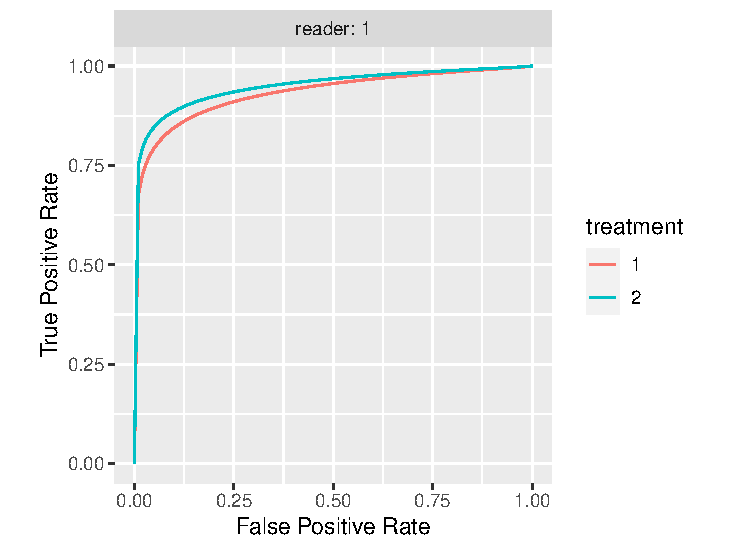
\includegraphics{MRMCaov_files/figure-latex/unnamed-chunk-25-1} \end{center}

\end{CodeChunk}

\textbf{SRMC ROC Curve Parameters}

\begin{CodeChunk}
\begin{CodeInput}
R> print(parameters(est))
\end{CodeInput}
\begin{CodeOutput}
# A tibble: 2 x 3
  Group$reader $treatment     a     b
  <fct>        <fct>      <dbl> <dbl>
1 1            1           1.70 0.537
2 1            2           1.85 0.503
\end{CodeOutput}
\end{CodeChunk}

\textbf{SRMC Test Results}

\begin{CodeChunk}
\begin{CodeInput}
R> summary(est)
\end{CodeInput}
\begin{CodeOutput}
Single-Reader Multi-Case Analysis of Variance
Data: VanDyke1
Factor types: Fixed Readers and Random Cases
Covariance method: jackknife

Experimental design: cases nested within reader 

Obuchowski-Rockette variance component and covariance estimates:

          Estimate Correlation
Error 0.0008371427          NA
Cov1  0.0004275632   0.5107412
Cov2  0.0000000000   0.0000000
Cov3  0.0000000000   0.0000000


95% CIs and tests for treatment binormal_auc pairwise differences:
  Comparison    Estimate     StdErr    CI.Lower    CI.Upper          z
1      1 - 2 -0.01765762 0.02862095 -0.07375366  0.03843841 -0.6169475
    p-value
1 0.5372694


Single reader 95% CIs:
  binormal_auc treatment reader     StdErr  CI.Lower  CI.Upper
1    0.9331609         1      1 0.03348356 0.8675343 0.9987874
2    0.9508185         2      1 0.02351885 0.9047224 0.9969146
\end{CodeOutput}
\end{CodeChunk}

\hypertarget{single-test-multi-case-analysis}{%
\section{Single-Test Multi-Case
Analysis}\label{single-test-multi-case-analysis}}

A single-test and single-reader multi-case (STMC) analysis involves a
single reader of multiple cases to estimate a reader performance metric
for one diagnostic test. An STMC analysis can be performed with a call
to \texttt{stmc()}.

\begin{figure}[h]
\begin{tcolorbox}[title=STMC Function]
\textbf{Syntax}
\begin{verbatim}
stmc(response, case, data, cov = jackknife)
\end{verbatim}
\begin{Description}
Returns an \code{stmc} class object of data that can be used to estimate a reader performance metric in a single-test and single-reader multi-case statistical analysis.
\end{Description}
\textbf{Arguments}
\begin{description}
\item[\code{response}:] object defining true case statuses, corresponding reader ratings, and a reader performance metric to compute on them.
\item[\code{case}:] variable containing the case identifiers for the \code{response} observations.
\item[\code{data}:] data frame containing the response and identifier variables.
\item[\code{cov}:] function \code{jackknife}, \code{unbiased}, or \code{DeLong} to estimate reader performance metric covariances.
\end{description}
\end{tcolorbox}
\end{figure}

The function is used similar to \texttt{mrmc()} but without the
\texttt{test} and \texttt{reader} arguments. In the following example,
an STMC analysis is performed with one of the tests and readers from the
\texttt{VanDyke} dataset.

\begin{CodeChunk}
\begin{CodeInput}
R> ## Subset VanDyke dataset by treatment 1 and reader 1
R> VanDyke11 <- subset(VanDyke, treatment == "1" & reader == "1")
R> 
R> ## Estimate ROC AUC for treatment 1 and reader 1
R> est <- stmc(binormal_auc(truth, rating), case, data = VanDyke11)
\end{CodeInput}
\end{CodeChunk}

\textbf{STMC ROC Curve}

\begin{CodeChunk}
\begin{CodeInput}
R> plot(est)
\end{CodeInput}


\begin{center}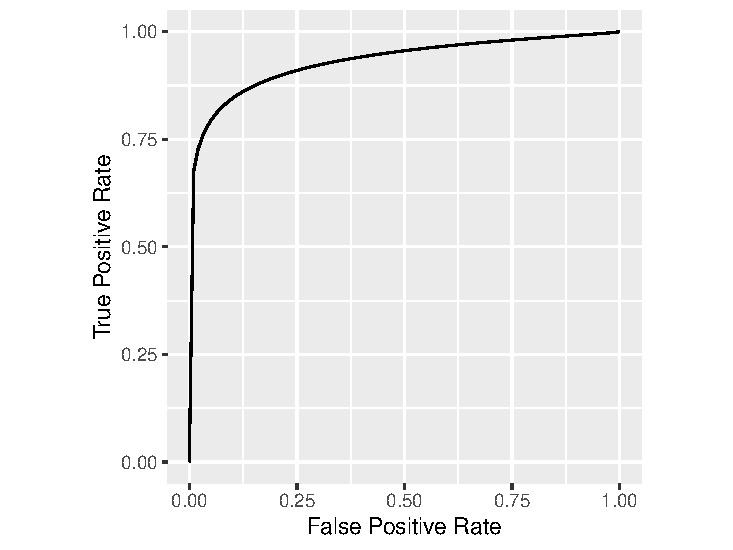
\includegraphics{MRMCaov_files/figure-latex/unnamed-chunk-28-1} \end{center}

\end{CodeChunk}

\textbf{STMC ROC Curve Parameters}

\begin{CodeChunk}
\begin{CodeInput}
R> print(parameters(est))
\end{CodeInput}
\begin{CodeOutput}
# A tibble: 1 x 2
      a     b
  <dbl> <dbl>
1  1.70 0.537
\end{CodeOutput}
\end{CodeChunk}

\textbf{STMC ROC AUC Estimate}

\begin{CodeChunk}
\begin{CodeInput}
R> summary(est)
\end{CodeInput}
\begin{CodeOutput}
binormal_auc       StdErr     CI.Lower     CI.Upper 
  0.93316085   0.03348356   0.86753427   0.99878743 
\end{CodeOutput}
\end{CodeChunk}

\hypertarget{roc-curves}{%
\section{ROC Curves}\label{roc-curves}}

ROC curves can be estimated, summarized, and displayed apart from a
multi-case statistical analysis with the \texttt{roc\_curves()}
function. Supported estimation methods include the empirical
distribution (default), binormal model, and binormal likelihood-ratio
model.

\hypertarget{curve-fitting}{%
\subsection{Curve Fitting}\label{curve-fitting}}

\begin{figure}[h]
\begin{tcolorbox}[title=ROC Curves Function]
\textbf{Syntax}
\begin{verbatim}
roc_curves(truth, rating, groups = list(), method = "empirical")
\end{verbatim}
\begin{Description}
Returns an \code{roc\_curves} class object of estimated ROC curves.
\end{Description}
\textbf{Arguments}
\begin{description}
\item[\code{truth}:] vector of true binary case statuses, with positive status taken to be the highest level.
\item[\code{rating}:] numeric vector of case ratings.
\item[\code{groups}:] list or data frame of grouping variables of the same lengths as \code{truth} and \code{rating}.
\item[\code{method}:] character string indicating the curve type as \code{"binormal"}, \code{"binormalLR"}, \code{"empirical"}, or \code{"trapezoidal"}.
\end{description}
\end{tcolorbox}
\end{figure}

A single curve can be estimated over all observations or multiple curves
estimated within the levels of one or more grouping variables. Examples
of both are given in the following sections using variables from the
\texttt{VanDyke} dataset referenced inside of calls to the
\texttt{with()} function. Alternatively, the variables may be referenced
with the \texttt{\$} operator; e.g., \texttt{VanDyke\$truth} and
\texttt{VanDyke\$rating}. Resulting curves from \texttt{roc\_curves()}
can be displayed with the \texttt{print()} and \texttt{plot()}
functions.

\hypertarget{single-curve}{%
\subsubsection{Single Curve}\label{single-curve}}

\begin{CodeChunk}
\begin{CodeInput}
R> ## Direct referencing of data frame columns
R> # curve <- roc_curves(VanDyke$truth, VanDyke$rating)
R> 
R> ## Indirect referencing using the with function
R> curve <- with(VanDyke, {
+   roc_curves(truth, rating)
+ })
R> plot(curve)
\end{CodeInput}


\begin{center}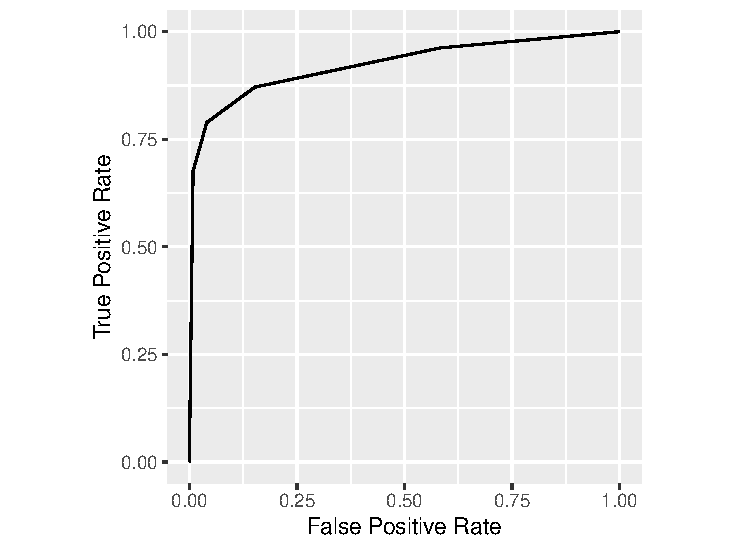
\includegraphics{MRMCaov_files/figure-latex/using_curves_one-1} \end{center}

\end{CodeChunk}

\hypertarget{multiple-curves}{%
\subsubsection{Multiple Curves}\label{multiple-curves}}

Multiple group-specific curves can be obtained from
\texttt{roc\_curves()} by supplying a list or data frame of grouping
variables to the \texttt{groups} argument. Groups will be formed and
displayed in the order in which grouping variables are supplied. For
instance, a second grouping variable will be plotted within the first
one.

\begin{CodeChunk}
\begin{CodeInput}
R> ## Grouped by reader
R> curves <- with(VanDyke, {
+   roc_curves(truth, rating,
+              groups = list(Reader = reader, Treatment = treatment))
+ })
R> plot(curves)
\end{CodeInput}


\begin{center}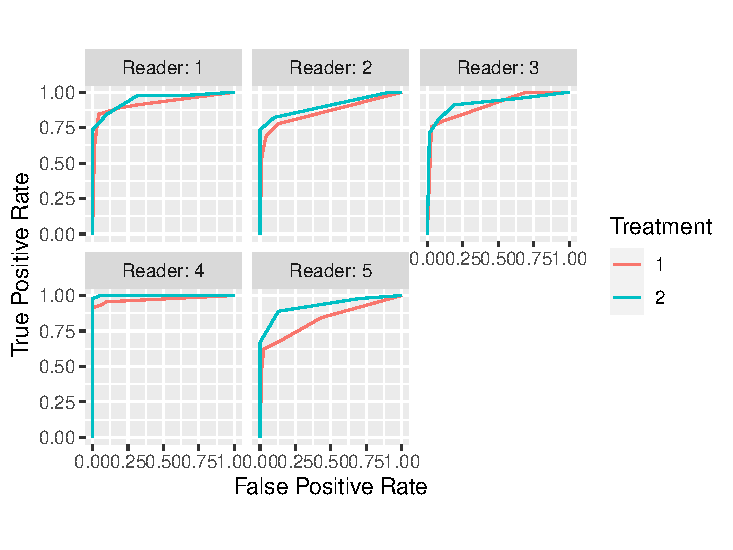
\includegraphics{MRMCaov_files/figure-latex/using_curves_reader-1} \end{center}

\end{CodeChunk}

\begin{CodeChunk}
\begin{CodeInput}
R> ## Grouped by treatment
R> curves <- with(VanDyke, {
+   roc_curves(truth, rating,
+              groups = list(Treatment = treatment, Reader = reader))
+ })
R> plot(curves)
\end{CodeInput}


\begin{center}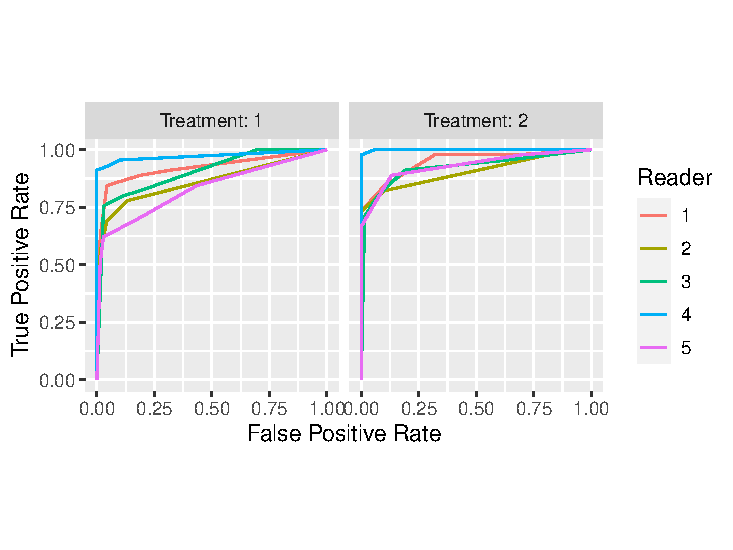
\includegraphics{MRMCaov_files/figure-latex/using_curves_treatment-1} \end{center}

\end{CodeChunk}

\hypertarget{parametric-curves}{%
\subsubsection{Parametric Curves}\label{parametric-curves}}

Estimated parameters for curves obtained with the binormal or binormal
likelihood-ratio models can be extracted as a data frame with the
\texttt{parameters()} function.

\begin{CodeChunk}
\begin{CodeInput}
R> ## Binormal curves
R> curves_binorm <- with(VanDyke, {
+   roc_curves(truth, rating,
+              groups = list(Treatment = treatment, Reader = reader),
+              method = "binormal")
+ })
R> params_binorm <- parameters(curves_binorm)
R> print(params_binorm)
\end{CodeInput}
\begin{CodeOutput}
# A tibble: 10 x 3
   Group$Treatment $Reader        a     b
   <fct>           <fct>      <dbl> <dbl>
 1 1               1       1.70e  0 0.537
 2 2               1       1.85e  0 0.503
 3 1               2       1.40e  0 0.561
 4 2               2       1.66e  0 0.447
 5 1               3       1.74e  0 0.635
 6 2               3       1.62e  0 0.488
 7 1               4       1.93e  0 0.202
 8 2               4       1.80e308 1    
 9 1               5       1.06e  0 0.464
10 2               5       1.73e  0 0.422
\end{CodeOutput}
\begin{CodeInput}
R> plot(curves_binorm)
\end{CodeInput}


\begin{center}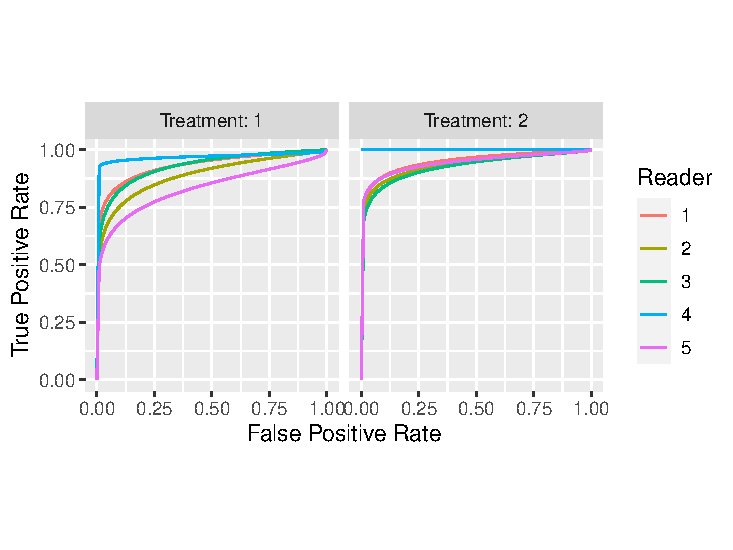
\includegraphics{MRMCaov_files/figure-latex/using_curves_binorm-1} \end{center}

\end{CodeChunk}

Estimates for different parameterizations of the binormal
likelihood-ratio model are additionally returned and include those of
the binormal model and the simplification of Pan and Metz
\citetext{\citeyear{Pan:1997:PBM}; \citealp{Metz:1993:PBR}} as well as
those of the bi-chi-squared model \citep{Hillis:2017:EBL}.

\begin{CodeChunk}
\begin{CodeInput}
R> ## Binormal likelihood-ratio curves
R> curves_binormLR <- with(VanDyke, {
+   roc_curves(truth, rating,
+              groups = list(Treatment = treatment, Reader = reader),
+              method = "binormalLR")
+ })
R> params_binormLR <- parameters(curves_binormLR)
R> print(params_binormLR)
\end{CodeInput}
\begin{CodeOutput}
# A tibble: 10 x 4
   Group$Treatment $Reader  Metz$d_a     $c bichisquared$la~   $theta binormal$a
   <fct>           <fct>       <dbl>  <dbl>            <dbl>    <dbl>      <dbl>
 1 1               1       2.13      -0.298             3.42 1.71e+ 0    1.71e+0
 2 2               1       2.35      -0.321             3.79 1.70e+ 0    1.87e+0
 3 1               2       1.73      -0.281             3.17 1.32e+ 0    1.40e+0
 4 2               2       0.0000680 -0.791            73.3  3.28e-11    4.84e-5
 5 1               3       0.0000725 -0.746            47.0  5.96e-11    5.18e-5
 6 2               3       2.08      -0.330             3.94 1.23e+ 0    1.65e+0
 7 1               4       0.000701  -0.932           797.   3.10e-10    4.96e-4
 8 2               4       0          1                 0    0         NaN      
 9 1               5       0.896     -0.507             9.37 5.94e- 2    6.66e-1
10 2               5       2.02      -0.553            12.1  2.17e- 1    1.49e+0
# ... with 1 more variable: binormal$b <dbl>
\end{CodeOutput}
\begin{CodeInput}
R> plot(curves_binormLR)
\end{CodeInput}


\begin{center}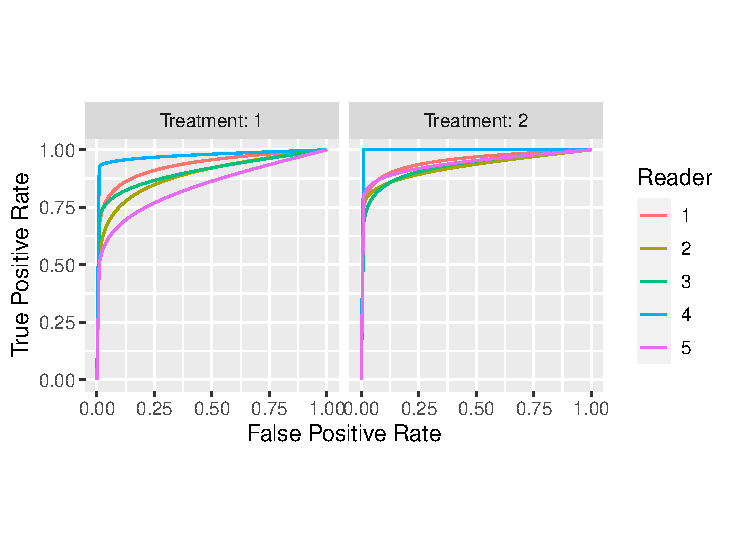
\includegraphics{MRMCaov_files/figure-latex/using_curves_binormLR-1} \end{center}

\end{CodeChunk}

\hypertarget{curve-points}{%
\subsection{Curve Points}\label{curve-points}}

Points on an ROC curve estimated with \texttt{roc\_curves()} can be
extracted with the \texttt{points()} function. True positive rates
(TPRs) and false positive rates (FPRs) on the estimated curve are
returned for a given set of sensitivity or specificity values or, in the
case of empirical curves, the original points. ROC curve points can be
displayed with \texttt{print()} and \texttt{plot()}.

\begin{figure}[h]
\begin{tcolorbox}[title=ROC Points Function]
\textbf{Syntax}
\begin{verbatim}
## Method for class 'roc_curves'`  
points(x, metric = "specificity", values = seq(0, 1, length = 101), ...)

## Method for class 'empirical_curves'`  
points(x, metric = "specificity", values = NULL, which = "curve", ...)
\end{verbatim}
\begin{Description}
Returns an \code{roc\_points} class object that is a data frame of false positive and true positive rates from an estimated ROC curve.
\end{Description}
\textbf{Arguments}
\begin{description}
\item[\code{x}:] object from \code{roc\_curves()} for which to compute points on the curves.
\item[\code{metric}:] character string specifying \code{"specificity"} or \code{"sensitivity"} as the reader performance metric to which \code{values} correspond.
\item[\code{values}:] numeric vector of values at which to compute ROC curve points, or \code{NULL} for default empirical values as determined by \code{which}.
\item[\code{which}:] character string indicating whether to use curve-specific observed values and 0 and 1 (\code{"curve"}), the combination of these values over all curves (\code{"curves"}), or only the observed curve-specific values (\code{"observed"}).
\end{description}
\end{tcolorbox}
\end{figure}

\begin{CodeChunk}
\begin{CodeInput}
R> ## Extract points at given specificities
R> curve_spec_pts <- points(curves, metric = "spec", values = c(0.5, 0.7, 0.9))
R> print(curve_spec_pts)
\end{CodeInput}
\begin{CodeOutput}
# A tibble: 30 x 3
   Group$Treatment $Reader   FPR   TPR
 * <fct>           <fct>   <dbl> <dbl>
 1 1               1         0.1 0.862
 2 1               1         0.3 0.908
 3 1               1         0.5 0.935
 4 2               1         0.1 0.843
 5 2               1         0.3 0.966
 6 2               1         0.5 0.978
 7 1               2         0.1 0.747
 8 1               2         0.3 0.821
 9 1               2         0.5 0.872
10 2               2         0.1 0.821
# ... with 20 more rows
\end{CodeOutput}
\begin{CodeInput}
R> plot(curve_spec_pts, coord_fixed = FALSE)
\end{CodeInput}


\begin{center}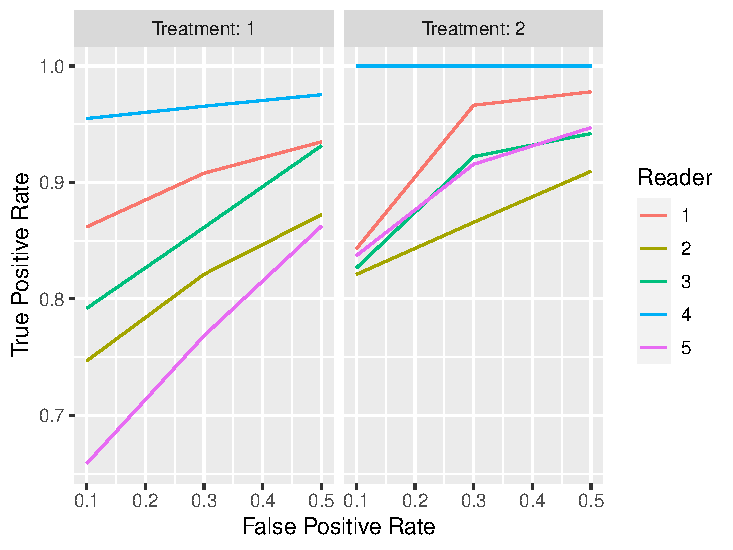
\includegraphics{MRMCaov_files/figure-latex/using_curves_points-1} \end{center}

\begin{CodeInput}
R> ## Extract points at given sensitivities
R> curve_sens_pts <- points(curves, metric = "sens", values = c(0.5, 0.7, 0.9))
R> print(curve_sens_pts)
\end{CodeInput}
\begin{CodeOutput}
# A tibble: 30 x 3
   Group$Treatment $Reader    FPR   TPR
 * <fct>           <fct>    <dbl> <dbl>
 1 1               1       0.0116   0.5
 2 1               1       0.0246   0.7
 3 1               1       0.254    0.9
 4 2               1       0        0.5
 5 2               1       0        0.7
 6 2               1       0.337    0.9
 7 1               2       0.0130   0.5
 8 1               2       0.0543   0.7
 9 1               2       0.609    0.9
10 2               2       0        0.5
# ... with 20 more rows
\end{CodeOutput}
\begin{CodeInput}
R> plot(curve_sens_pts, coord_fixed = FALSE)
\end{CodeInput}


\begin{center}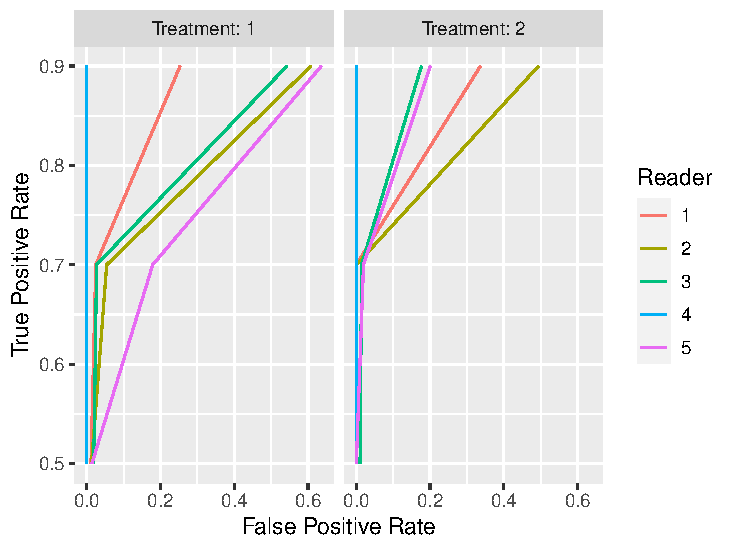
\includegraphics{MRMCaov_files/figure-latex/using_curves_points-2} \end{center}

\end{CodeChunk}

\hypertarget{mean-curves}{%
\subsection{Mean Curves}\label{mean-curves}}

A mean ROC curve from multiple group-specific curves returned by
\texttt{roc\_curves()} can be computed with the \texttt{means()}
function. Curves can be averaged over sensitivities, specificities, or
binormal parameters \citep{Chen:2014:ARO}. Averaged curves can be
displayed with \texttt{print()} and \texttt{plot()}.

\begin{figure}[h]
\begin{tcolorbox}[title=ROC Means Function]
\textbf{Syntax}
\begin{verbatim}
## Method for class 'roc_curves'
mean(x, ...)`

## Method for class 'binormal_curves'
mean(x, method = "points", ...)
\end{verbatim}
\begin{Description}
Returns an \code{roc\_points} class object.
\end{Description}
\textbf{Arguments}
\begin{description}
\item[\code{x}:] object from \code{roc\_curves()} for which to average over the curves.
\item[\code{method}:] character string indicating whether to average binormal curves over \code{"points"} or \code{"parameters"}.
\item[\code{...}:] optional arguments passed to \code{points()}, including at which \code{metric} (\code{"sensitivity"} or \code{"specificity"}) values to average points on the ROC curves.
\end{description}
\end{tcolorbox}
\end{figure}

\begin{CodeChunk}
\begin{CodeInput}
R> ## Average sensitivities at given specificities (default)
R> curves_mean <- mean(curves)
R> print(curves_mean)
\end{CodeInput}
\begin{CodeOutput}
# A tibble: 20 x 2
      FPR   TPR
 *  <dbl> <dbl>
 1 0      0    
 2 0      0.402
 3 0.0145 0.686
 4 0.0290 0.762
 5 0.0435 0.790
 6 0.0580 0.802
 7 0.0725 0.813
 8 0.101  0.835
 9 0.116  0.844
10 0.130  0.852
11 0.159  0.862
12 0.188  0.872
13 0.319  0.904
14 0.362  0.912
15 0.435  0.925
16 0.638  0.956
17 0.667  0.961
18 0.696  0.966
19 0.913  0.992
20 1      1    
\end{CodeOutput}
\begin{CodeInput}
R> plot(curves_mean)
\end{CodeInput}


\begin{center}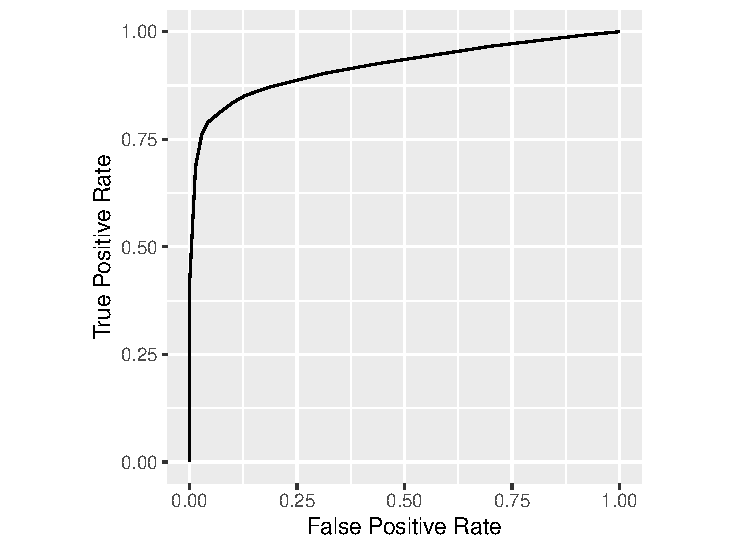
\includegraphics{MRMCaov_files/figure-latex/using_curves_mean_spec-1} \end{center}

\end{CodeChunk}

\begin{CodeChunk}
\begin{CodeInput}
R> ## Average specificities at given sensitivities
R> curves_mean <- mean(curves, metric = "sens")
R> print(curves_mean)
\end{CodeInput}
\begin{CodeOutput}
# A tibble: 23 x 2
       FPR   TPR
 *   <dbl> <dbl>
 1 0       0    
 2 0.00698 0.511
 3 0.00804 0.556
 4 0.00899 0.578
 5 0.00995 0.6  
 6 0.0109  0.622
 7 0.0214  0.667
 8 0.0280  0.689
 9 0.0358  0.711
10 0.0450  0.733
# ... with 13 more rows
\end{CodeOutput}
\begin{CodeInput}
R> plot(curves_mean)
\end{CodeInput}


\begin{center}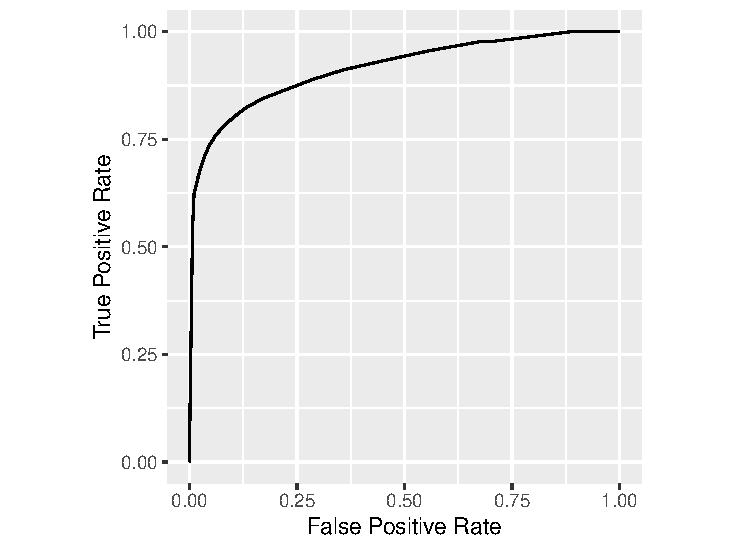
\includegraphics{MRMCaov_files/figure-latex/using_curves_mean_sens-1} \end{center}

\end{CodeChunk}

\hypertarget{reader-performance-metrics}{%
\section{Reader Performance Metrics}\label{reader-performance-metrics}}

The reader performance metrics described previously for use with
\texttt{mrmc()} and related functions to analyze multi and single-reader
multi-case studies can be applied to truth and rating vectors as
stand-alone functions. This enables estimation of performance metrics
for other applications, such as predictive modeling, that may be of
interest.

\hypertarget{roc-curve-metrics}{%
\subsection{ROC Curve Metrics}\label{roc-curve-metrics}}

AUC, partial AUC, sensitivity, and specificity are estimated below with
an empirical ROC curve. Estimates with binormal and binormal
likelihood-ratio curves can be obtained by replacing \texttt{empirical}
in the function names with \texttt{binormal} and \texttt{binormalLR},
respectively.

\begin{CodeChunk}
\begin{CodeInput}
R> ## Total area under the empirical ROC curve
R> empirical_auc(VanDyke$truth, VanDyke$rating)
\end{CodeInput}
\begin{CodeOutput}
[1] 0.9229791
\end{CodeOutput}
\begin{CodeInput}
R> ## Partial area for specificity from 0.7 to 1.0
R> empirical_auc(VanDyke$truth, VanDyke$rating, partial = "spec", min = 0.70,
+               max = 1.0)
\end{CodeInput}
\begin{CodeOutput}
[1] 0.2499923
\end{CodeOutput}
\begin{CodeInput}
R> ## Partial area for sensitivity from 0.7 to 1.0
R> empirical_auc(VanDyke$truth, VanDyke$rating, partial = "sens", min = 0.70,
+               max = 1.0)
\end{CodeInput}
\begin{CodeOutput}
[1] 0.2262129
\end{CodeOutput}
\begin{CodeInput}
R> ## Sensitivity for given specificity
R> empirical_sens(VanDyke$truth, VanDyke$rating, spec = 0.8)
\end{CodeInput}
\begin{CodeOutput}
[1] 0.8812346
\end{CodeOutput}
\begin{CodeInput}
R> ## Sensitivity for given specificity
R> empirical_spec(VanDyke$truth, VanDyke$rating, sens = 0.8)
\end{CodeInput}
\begin{CodeOutput}
[1] 0.94434
\end{CodeOutput}
\end{CodeChunk}

\hypertarget{binary-metrics-1}{%
\subsection{Binary Metrics}\label{binary-metrics-1}}

Sensitivity and specificity for binary ratings are available with the
\texttt{binary\_sens()} and \texttt{binary\_spec()} functions as
demonstrated in the next example based on a binary rating created from
the numeric one in the \texttt{VanDyke} dataset.

\begin{CodeChunk}
\begin{CodeInput}
R> ## Create binary classification
R> VanDyke$binary_rating <- VanDyke$rating >= 3
R> 
R> ## Sensitivity
R> binary_sens(VanDyke$truth, VanDyke$binary_rating)
\end{CodeInput}
\begin{CodeOutput}
[1] 0.8711111
\end{CodeOutput}
\begin{CodeInput}
R> ## Specificity
R> binary_spec(VanDyke$truth, VanDyke$binary_rating)
\end{CodeInput}
\begin{CodeOutput}
[1] 0.8478261
\end{CodeOutput}
\end{CodeChunk}

\hypertarget{conclusion}{%
\section{Conclusion}\label{conclusion}}

\pkg{MRMCaov} brings a new statistical package for MRMC analysis to the
\proglang{R} software environment and its large community of users. The
package enables comparison of diagnostic tests with an interactive
interface and flexible options for performance metrics, study designs,
covariance estimation methods, and statistical estimation and testing of
performance. A demonstration of features currently implemented in the
package is provided in this paper. Proper statistical methods and
readily available software are crucial for the evaluation and comparison
of multi-reader multi-case studies. The \pkg{MRMCaov} software is
designed to help ensure the application of such methods.

\renewcommand\refname{References}
\bibliography{../src/bibliography.bib}



\end{document}
